\chapter{CSA}

\label{chap:CSA}

Card Sorting Analysis (CSA) was developed at Graz University of
Technology as part of the course Information Architecture and Web
Usability. It allows users to analyse the results of card sorting
studies, but does not offer the capabilities to create an online card
sorting study within the program. It is also worth mentioning, that
CSA can only be launched after install R via console or after
installing R and RStudio via the RStudio GUI.


\begin{figure}[tp] 
\centering
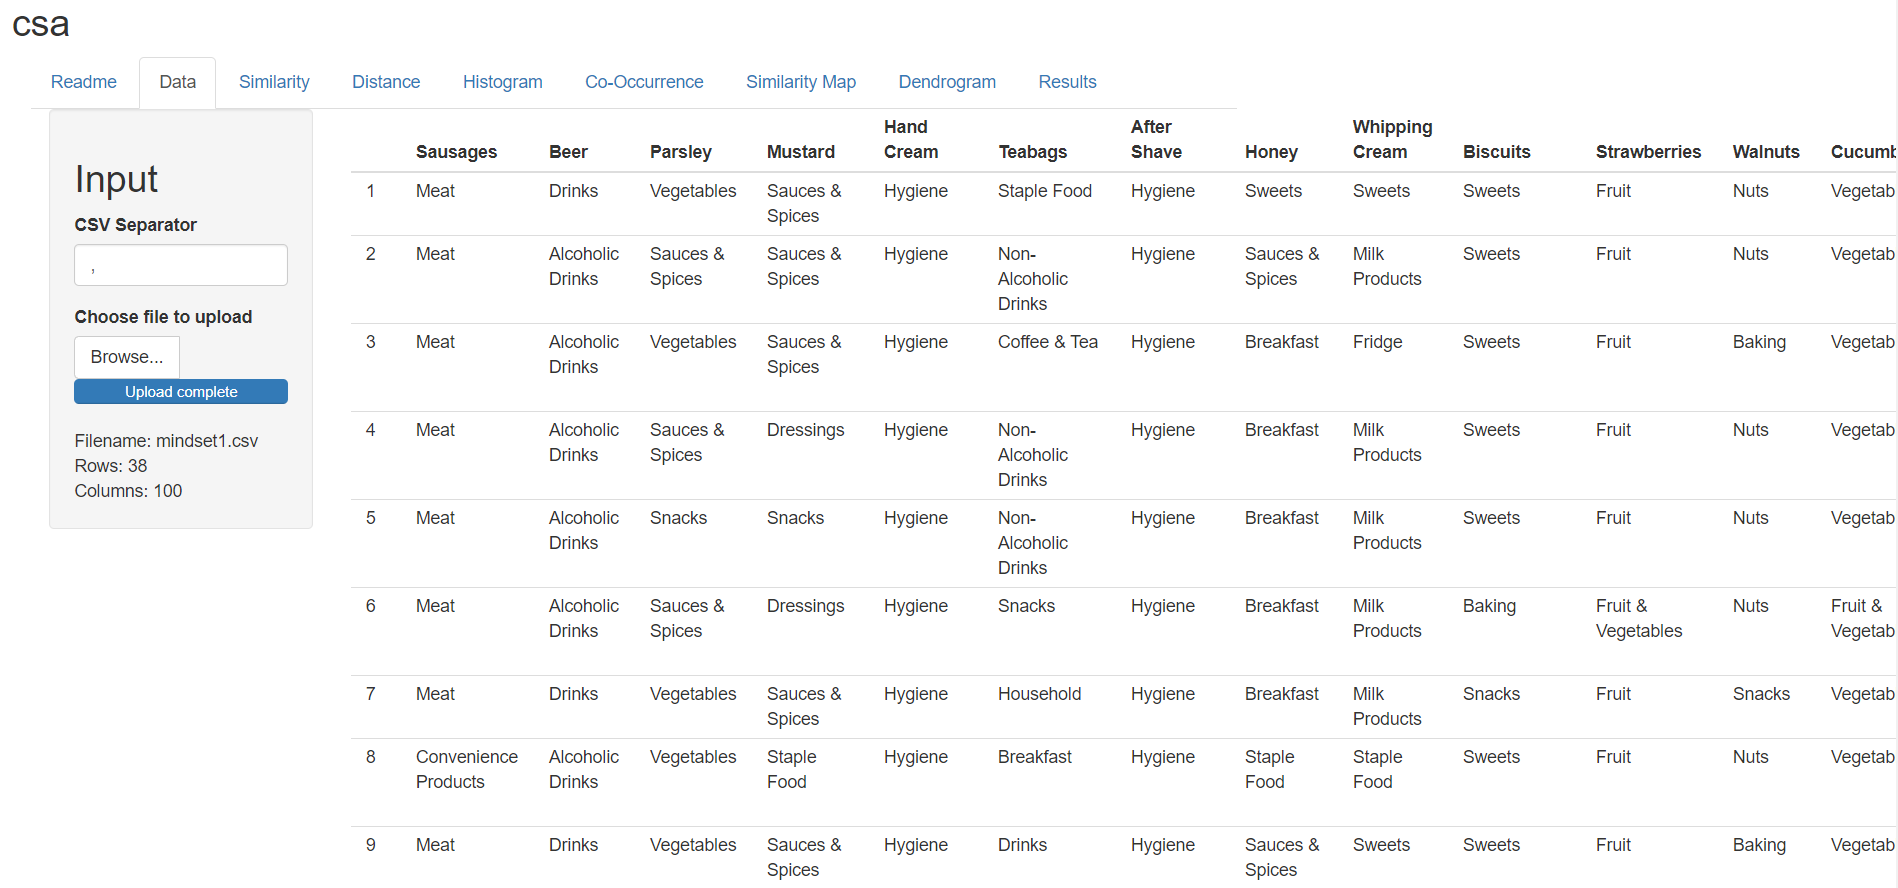
\includegraphics[keepaspectratio,width=\linewidth,height=\halfh]{images/csa-data.png}
\caption[CSA Application] { This is the base view within CSA
once data is imported with a .csv file.
\imgcredit{Screenshot was captured by Markus Ruplitsch using
\textcite{CSA}.} }
\label{fig:CSA1}
\end{figure}



\section{Business Model}

CSA is not publicly available. The only way to gain access is via contacting 
Prof.\ Keith Andrews.


\section{Card Sorting}

Just like the other analysis tools before, CSA does not support online card 
sorting and has to be used in conjuction with another form of card sorting, 
either physical or online. The results can then be imported to CS via a .csv 
file.


\section{Analytics}

Before starting CSA, it is necessary to install R, and RStudio if one does not 
like using command line arguments. Even for tech-savy people, it will take a 
while to install all necessary R packages and set up a working directory. It 
stands to reason, that the installation process will be extremely difficult for 
users who have no experience programming, or working with programs without a 
professionally designed user face.

After importing data as a .csv file, CSA offers a variety of visualizations. 
These visualizations can be accessed via a Menu bar at the top and can be 
exported as .csv, .svg or .png, depending on the type of visualization. The 
visualizations offered by CSA are: similarity matrix, distance matrix, distance 
histogram, co-occurrence matrix, similarity map, dendrogram and a results 
table. 


\begin{figure}[tp] 
\centering
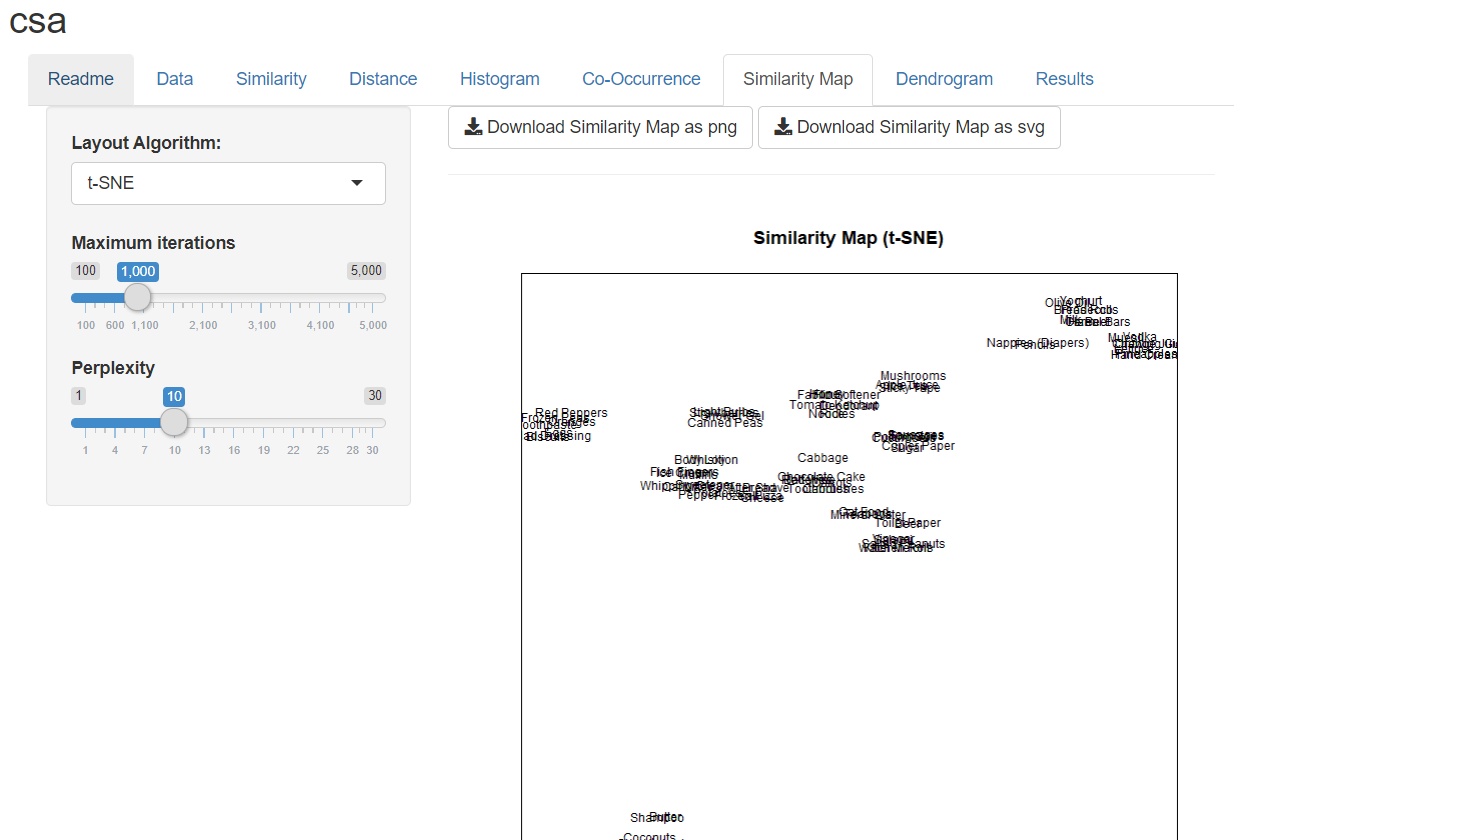
\includegraphics[keepaspectratio,width=\linewidth,height=\halfh]{images/csa-similarity.png}
\caption[CSA Similarity Map] { This screenshot shows a similarity map over
all cards that are used for analytics.
\imgcredit{Screenshot was captured by Markus Ruplitsch using
\textcite{CSA}.} }
\label{fig:CSA2}
\end{figure}

\begin{figure}[tp] 
\centering
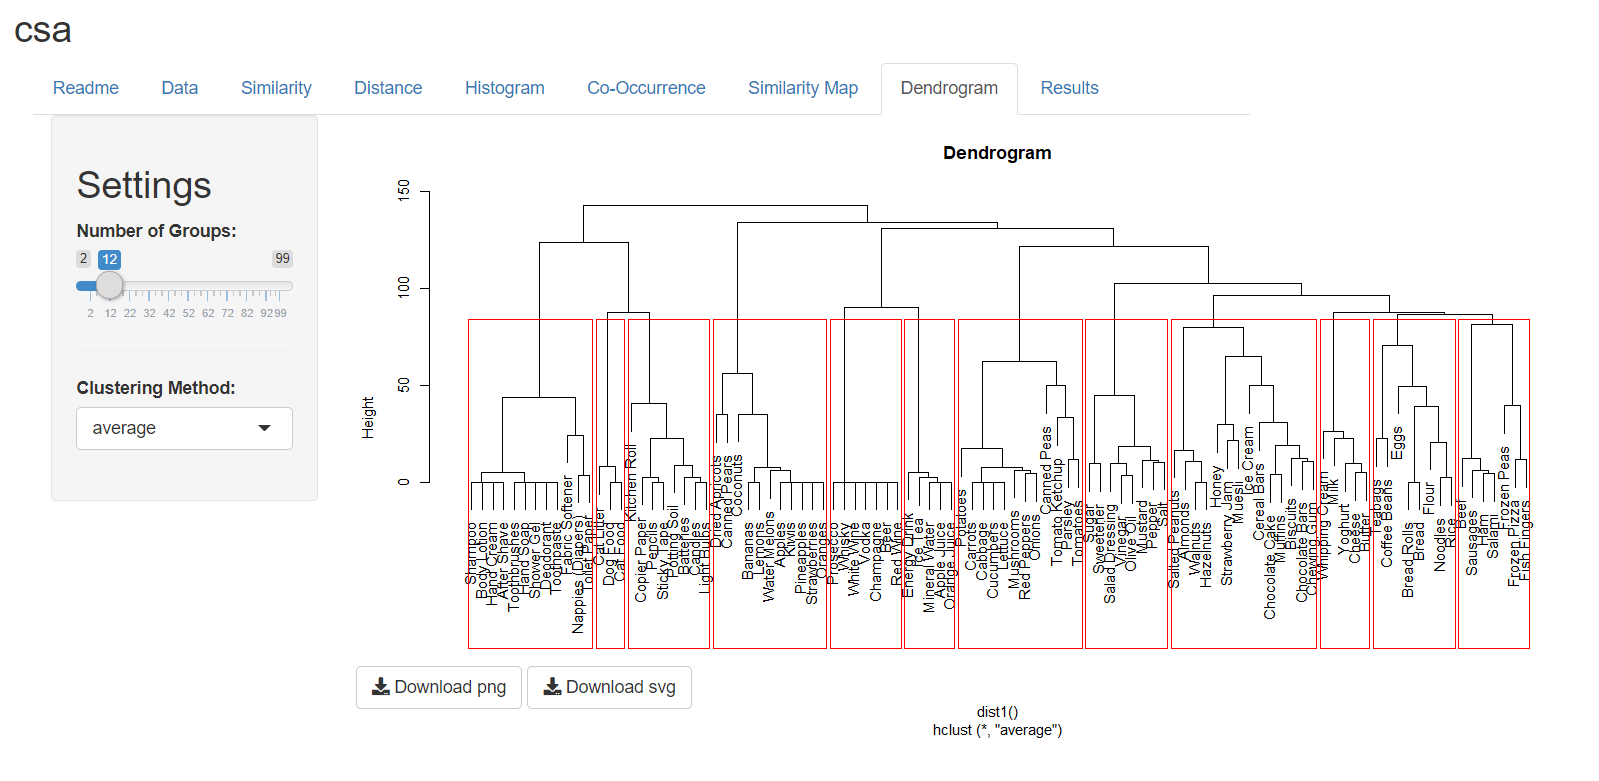
\includegraphics[keepaspectratio,width=\linewidth,height=\halfh]{images/csa-dendrogram.png}
\caption[CSA Dendrogram] { This screenshot shows a dendrogram 
for the average link of cards which is used for analytics.
\imgcredit{Screenshot was captured by Markus Ruplitsch using
\textcite{CSA}.} }
\label{fig:CSA3}
\end{figure}

\begin{table}[tp]
\centering
\begin{tabularx}
{\linewidth}{|l|X|}
\hline \textbf{Feature/Characteristic} & \textbf{Availability in Casolysis} \\ 
\hline Card Sorting & None. Paper Cards or other tools needed. \\ 
\hline Card Limit & None. \\
\hline Participant Limit & None. \\
\hline Analytics & Analytics with 7 different types of visualizations. \\ 
\hline Documentation & None. \\
\hline Business Model & Not publicly available \\
\hline Import formats & .csv\\ 
\hline Export formats & .csv, .png, .svg \\ 
\hline Sub-Categories & Not really supported, but can be used \\ 
\hline Playback of user-sessions & No. \\ 
\hline Data preparation & No. Has to be done before inporting the .csv file \\ 
\hline
\end{tabularx} 
\caption[Feature summary of CSA] 
{ 
This table summarizes all the features and characteristics of CSA
to provide an easy to read overview.
}
\label{tab:features-CSA}
\end{table}

\section{Summary \& Ratings}
While the analytics capabilities of CSA are quite extensive, there are some 
major problems when it comes to using it. First of all, it will be extremely 
hard for new users to install it if they do not have a background in computer 
science or are highly tech savy. This is not necessarily the applications 
fault, but rather comes with the fact that it is an R application and can only 
be launched via R or RStudio. Additionally, this is not made easier by the 
complete lack of documentation, aside from a small readme file in the main 
directory. Because of this, we decided to give CSA a 0 for simplicity and 
documentation. 

Secondly, most people will never use CSA because it is not publicly available. 
Wihle we just as well, could have given CSA a 5 for its business model, since 
it is free, we decided to take into account the fact that the majority of people
will never hear of CSA, or be able access to it. These flaws lead to CSA 
having the lowest average score of only 1.0.





\begin{table}[tp] 
\centering 
\begin{tabularx}{\linewidth}{|X|X|X|X|X|}
\hline
Simplicity & Documentation & Features & Business Model & Average \\ 
\hline 
0 & 0 & 4 & 0 & 1.0 \\ 
\hline 
\end{tabularx} 
\caption[Ratings for CSA] {
Ratings for CSA including the average rating.
} 
\label{tab:rating-CSA}
\end{table}







